
\begin{question}
Consider the following time series on Australian monthly gas production:

\begin{figure}[H]
\centering
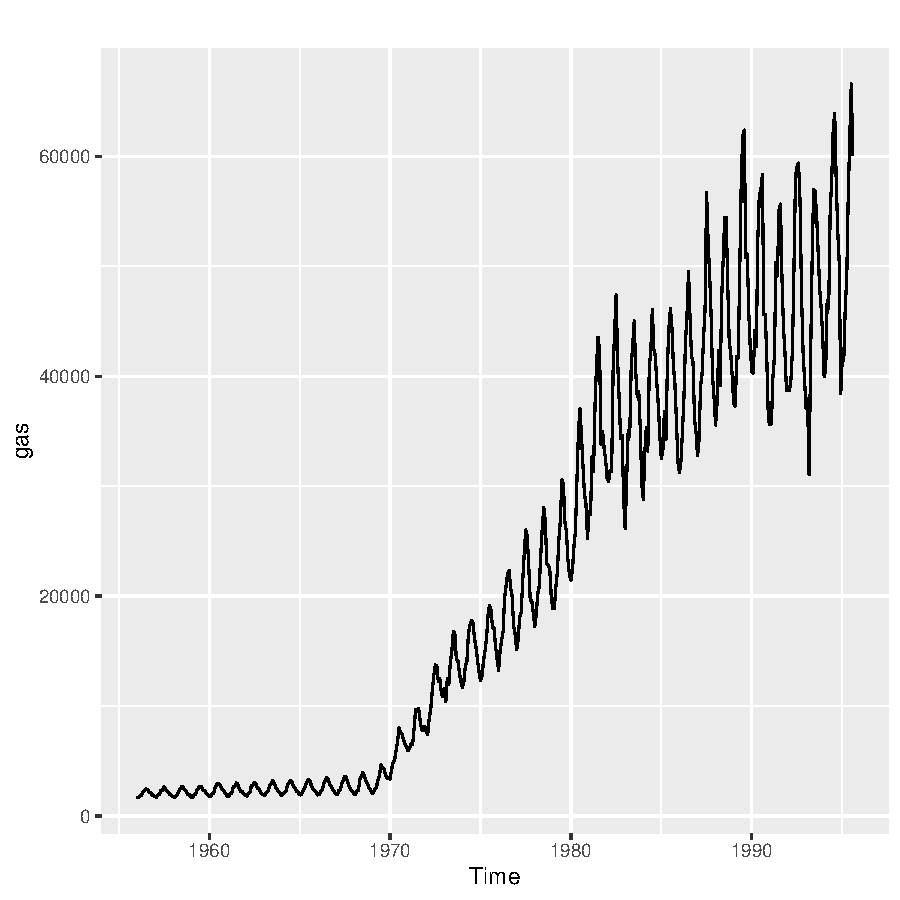
\includegraphics{unnamed-chunk-1-1.pdf}
\caption{plot of chunk unnamed-chunk-1}
\end{figure}

We have applied Box-Cox tranformation with different parameters:

\begin{figure}[H]
\centering
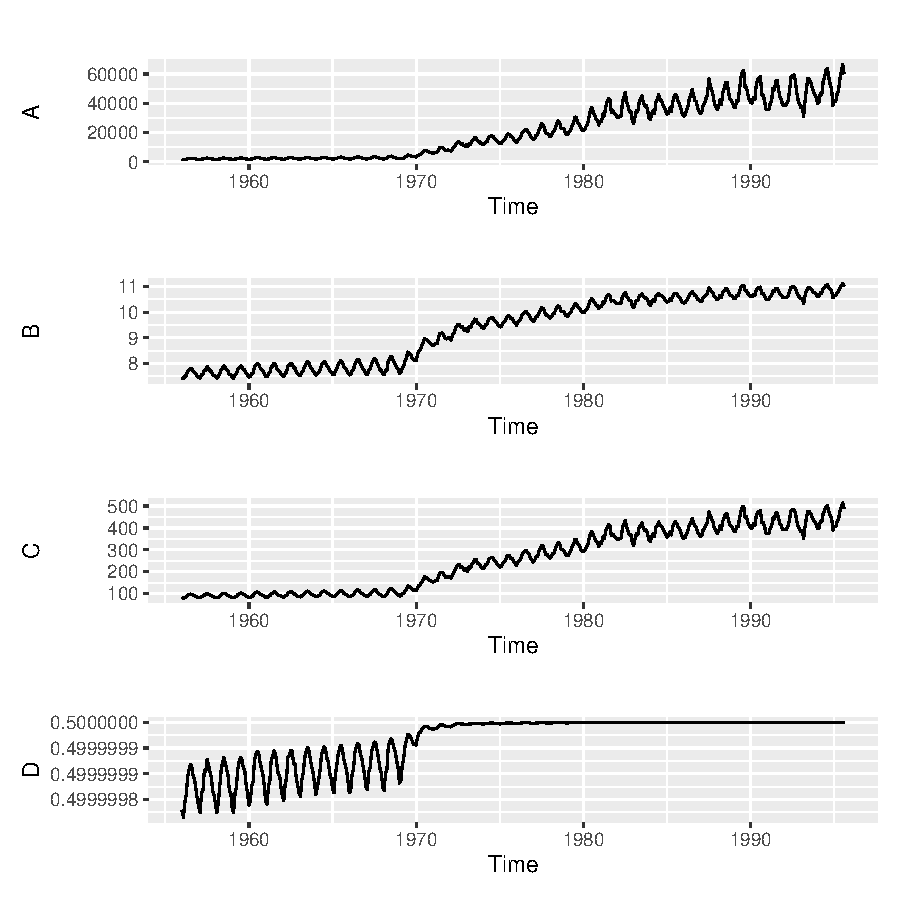
\includegraphics{unnamed-chunk-2-1.pdf}
\caption{plot of chunk unnamed-chunk-2}
\end{figure}

\begin{enumerate}
\def\labelenumi{\arabic{enumi}.}
\item
  \(\lambda=-2\)
\item
  \(\lambda=0\)
\item
  \(\lambda=1\)
\item
  \(\lambda=0.5\)
\end{enumerate}

Write down in the solution the sequence of numbers without spaces or delimeters corresponding to parameters of Box-Cox transformation \(\lambda_A,\lambda_B,\lambda_C,\lambda_D\) applied in each case (e.g.~4231).
\end{question}

\begin{solution}
Suppose \(y^{bc}\) is transformed data. If \(\lambda=0\), the transformation is equivalent to \(y^{bc}=\ln(y)\), if \(\lambda=1\) it's \(y^{bc}=y\), if \(\lambda=0.5\) it's \(y^{bc}=\sqrt{y}\), if \(\lambda=-2\) it's \(y^{bc}=y^{-2}\).
\end{solution}

